\chapter{Romano: IO Load Balancer}
\label{ROMANO}

%% Motivation
The cloud computing paradigm shift is built on virtualization.
Most IT organizations and cloud service providers have deployed virtualized data centers in an effort to consolidate workloads, streamline management, reduce costs and increase utilization.
Still, overall costs for {\em storage management} have remained stubbornly high.
Over its lifetime, managing storage is often four times more expensive than its initial procurement~\cite{merrill:2009}.
The annualized total cost of storage for virtualized systems is often three times more than server hardware and seven times more than networking-related assets~\cite{simpson:2010}.

A key enabler for virtualization adoption is ability for a virtual machine (VM) to be efficiently migrated across compute hosts at run time~\cite{clark:2005, wood:2007, nelson:2005}.
Consequently, VM live migration has been utilized to perform active performance management in commercial products for some time~\cite{vmware:2006}. 
Similarly, virtualization offers unprecedented dynamic control over storage resources, allowing both VMs and their associated virtual disks to be placed dynamically and migrated seamlessly around the physical infrastructure~\cite{mashtizadeh:2011}.

However, it is well-known that storage data associated with a VM is much harder to migrate compared to CPU and Memory state. 
Virtual disk migration time is typically a function of virtual disk size, size of the working set, source and destination storage state and capability, etc~\cite{mashtizadeh:2011}. 
Migration can take anywhere from tens of minutes to a few hours depending on those parameters.

Given the high expense of data migration, intelligent and automatic storage performance management has been a relevant but difficult research problem~\cite{gulati:2010, gulati:2011}. 
Virtualized environments can be extremely complex, with diverse and mixed workloads sharing a collection of heterogeneous storage devices. 
Such environments are also dynamic, as new devices, hardware upgrades, and other configuration changes are rolled out. 
Our goal of supporting heterogeneity is critical since data center operators want to keep the flexibility of buying the cheapest hardware available at any given time.

%% Problem
The key to automated management of storage lies in the ability to predict the performance of a workload on a given storage system.
Without it, an experienced user must determine manually if migrating a virtual disk is beneficial, a complicated task. 
Previous work~\cite{gulati:2010, gulati:2011} has relied on a heuristic model derived from empirical data.

When considering automated load balancing, the simplest approach would be to observe utilization of all data stores and offload a virtual disk from the most heavily loaded data store to the least heavily loaded data store.

There are several problems with this approach but the main problem is the unpredictability of the benefit of the moves. 
In fact, there exists no guarantee that the moves will even be beneficial. Storage systems do not react to different workloads in a homogeneous manner. 
A workload may stress one storage system significantly more than the other depending on the storage system configurations and optimizations.

The second problem is the workload interference.
When multiple workloads are placed into a single storage systems, their effect on the storage system is not simply additive. While some workloads can be placed onto a single storage system and work with minimum interference, some experience huge performance hits.

Romano prediction model takes into account this heterogeneous response of storage systems and the interference between workloads improving the prediction accuracy by over 80\%. Once these problems are recognized, it is obvious that the load balancing is no longer a bin packing problem as suggested by previous works~\cite{gulati:2010, gulati:2011, singh:2008}.
Therefore, we introduce a new load balancing algorithm based on simulated annealing~\cite{kirkpatrick:1983} that optimizes the overall performance in a stochastic manner.
We show that Romano is capable of reducing the performance variance by 82\% and reduce the maximum latency observed by 78\%.

Romano makes following contributions.
\begin{description}
\item[Accuracy] Romano residuals are reduced 80\% on average compared to previous techniques. 
Furthermore, the residual is unbiased and does not propagate with recursive predictions.
\item[Robustness] Romano is able to specify the prediction interval which satisfies a specified confidence level.
We show that the resulting prediction interval captures real performance with surprising accuracy.
\item[Flexibility] Different storage systems have different response characteristics to different workloads. 
Romano captures these differences by quantifying the effect of workload characteristics as well as the interactions of those characteristics on a given storage system.
\item[Optimization] Romano load-balancing algorithm avoids having system state stuck in a local optimum, instead identifying a global pseudo-optimal state through recursive prediction. 
At the same time, it also ensures that the most beneficial migrations are performed first to maximize the benefit.
\end{description}

We have prototyped \romano on VMware's ESXi and vCenter Server products. 
Minimal changes were made to the ESXi hypervisor to collect additional stats for vCenter where the core of \romano is implemented.

\section{Romano Design}

\begin{figure}[!t]
\centering
\begin{tikzpicture}[node distance = 2in, auto]
\node[clod,
  minimum height=1.1in,
  minimum width=3in
  ] (VDP) {Virtual Disk Pool};
\node[block,
  text width=13em,
  node distance=1.3in,
  below of=VDP,
  minimum height=1in,
  minimum width=5.5in
  ] (RM) {
  \begin{minipage}[t][0.8in]{6in}
    Resource Manager
  \end{minipage}
  };
\node[block,
  node distance=0.1in,
  below of=RM
  ] (LB) {Romano \\ Load \\ Balancer};
\node[block,
  right of=LB,
  node distance = 1.8in
  ] (RPM) {Romano \\ Performance \\ Model};
\node[block,
  left of=LB,
  node distance = 1.8in
  ] (RIM) {Romano \\ Aggregation \\ Model};
\node[clod,
  node distance=1.3in,
  minimum height=1.1in,
  minimum width=3in,
  below of=RM
  ] (DSP) {Data Store Pool};
\path[line] (VDP) -- (RM);
\path[line] (RM) -- (DSP);
\end{tikzpicture}

\captionsetup{format=myformat}
\caption{High level view of Romano.
Romano maps virtual disks onto pool of data stores to satisfy the load balancing policy.
}
\label{ov}
\end{figure}

Romano is a generic framework that allows automated load balancing of the virtual disks in a heterogeneous storage environment. 
Specifically, Romano predicts the storage performance using statistical techniques allowing the systems to relocate the virtual disks without the human
intervention.

\figurename~\ref{ov} shows an overview of Romano framework.
Romano sits within the Resource Manager which maps physical storage resources to the virtual disks.
Romano framework consists of \emph{Romano Performance Model}, \emph{Romano Aggregation Model} and a \emph{Romano Load Balancer}.
Romano Performance Model was described in Chapter~\ref{SPM}.
Romano Aggregation Model predicts the characteristics of multiple independent workloads when they are aggregated on a single data store.
Romano Load Balancer balances the workloads across heterogeneous data stores such that the mean and maximum latency observed by the virtual disks are minimized.

These components will be described in detail next.

\section{Romano Aggregation Model}
Predicting the performance of a data store given a workload is not always enough.
If the data store is already running different workloads, we need to figure out what the characteristics of aggregated workload will be.

In Basil, this is done by simply adding their workload parameter $\omega$~\cite{gulati:2011}.
This made sense under their assumption that all data stores react to different workloads in a similar manner.
Since $\omega$ represents the amount of work a data store has to process, aggregating workloads only involve addition of $\omega$'s.

Romano's workload model is a tuple of different combinations of characteristics.
It makes more sense to aggregate each characteristic separately.
In our closed loop assumption, aggregation of workloads does not affect the number of IOs each workload keeps in the system.
Therefore we can safely assume that the \emph{Outstanding IO}s~($\OIO$) will simply be added.

However, \emph{Size}~($\SIZE$) and \emph{Read Ratio}~($\READ$) can not be simply added together.
It needs to be averaged based on ratio of number of requests seen by the two workloads that are being aggregated.
Pesto weights each value by their $\OIO$, assuming that higher $\OIO$ means higher rate of requests.
However, $\OIO$ can be highly independent of arrival rate.
For example, imagine a process that generates 5 IO requests and issues additional IO whenever a request completes.
The arrival rate will only depend on the service rate of the requests and not on outstanding IOs which would be fixed at 5.
For Romano this weight to be used for averaging is already available as the inverse of \emph{LQ-slope}, which represents the throughput~($T$) from our performance model in Equation \ref{rpmf:eq}.

The \emph{Random}~($\RAND$) is tricky because the randomness of access cannot be defined per IO request and cannot be simply averaged.

\begin{figure}[!t]
\centering
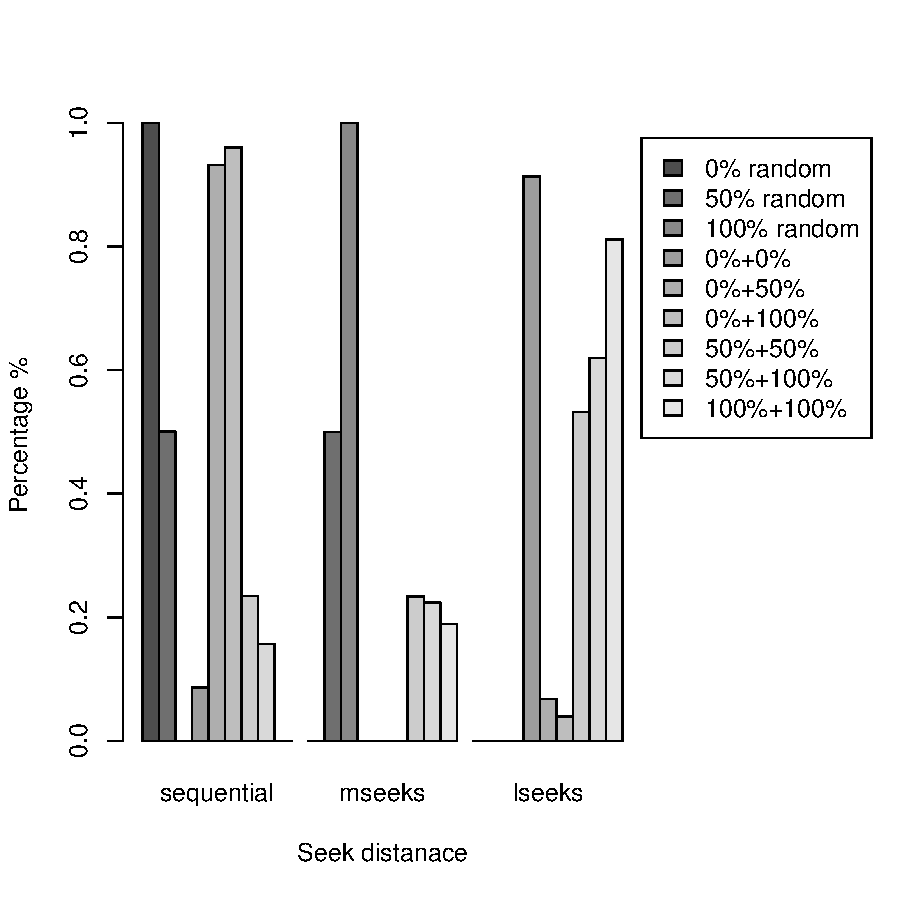
\includegraphics[width=0.8\textwidth]{figure/seek_profile.pdf}
\captionsetup{format=myformat}
\caption{Seek profile of different workloads.
Each color represents different mix of $\RAND$ for workload with $\SIZE=4\mathit{KB}$, $\READ=100\%$ read, $\OIO=1$.
\emph{mseeks} represents seeks done within a virtual disk and \emph{lseeks} represents seeks done across the virtual disks.}
\label{seekpr}
\end{figure}
\figurename~\ref{seekpr} shows the changes in the seek profile as you mix 0\%, 50\% and 100\% random workloads on E1 data store.
Our measurements show that the \emph{LQ-slope} for these workloads are 0.476, 17.6 and 35.8 respectively.
Therefore, the throughput~($T$), of these workloads are 2100.52, 56.77 and 27.93 respectively.

Note that \emph{mseeks} represents seeks within a virtual disk while \emph{lseeks} represents seeks across the virtual disks.
If we define the \emph{randomness} of the workloads as percentage of the seeks, the effect of aggregation is completely non-linear and hard to predict.
However, we make the following observations.
\begin{enumerate}
\item Mixing sequential workload and non-sequential workloads results in very low \emph{mseeks}.
\item The number of lseeks is determined by the lower throughput of two workloads.
\item The number of lseeks reduces the sequential and mseeks by the ratio of their average $T$.
\end{enumerate}
More formally,
\begin{align}
\overline{seq}&=\frac{\mathit{seq}_1T_1*\mathit{seq}_2T_2}{T_1+T_2}\label{r1}\\
\mathit{seq}&=\overline{seq}-(\overline{seq}*\mathit{\%lseek})\label{r2}\\
\mathit{\%lseek}&=\frac{\min(T_1,T_2)}{T_1+T_2}*2*\overline{seq}\label{r3}
\end{align}
which can be solved for ${\RAND}=1-\mathit{seq}$ to be:
\begin{equation}\label{randFun}
R_{\mathit{aggr}}=f_{\RAND}({\RAND}_1, {\RAND}_2, T_1, T_2)
=1-\frac{T_1T_2(1-{\RAND}_1)(1-{\RAND}_2)(1+2\min(T_1,T_2))}{T_1+T_2}.
\end{equation}
Equation \ref{r1} is a simple throughput weighted average of the $sequential\%$ representing average $mseeks$.
However, this does not account for additional seeks due to serving multiple virtual disks.
Therefore Equation \ref{r2} subtracts the amount of $lseeks$ from the $sequential\%$.
Note that the $\%lseek$ in the equation represents the percentage of $lseek$s.
Intuitively, the storage system is typically serving the high throughput workload and occasionally seeks to low throughput workload which causes the $lseek$.
Therefore, Equation \ref{r3} calculates the amount of $lseeks$ which is proportional to the ratio between the low throughput and the total throughput.
This value is multiplied by $2*\overline{seq}$ since almost every $lseek$ between the sequential workload is matched by a $lseek$ in the opposite direction to serve both virtual disks.

\begin{figure}[!t]
\centering
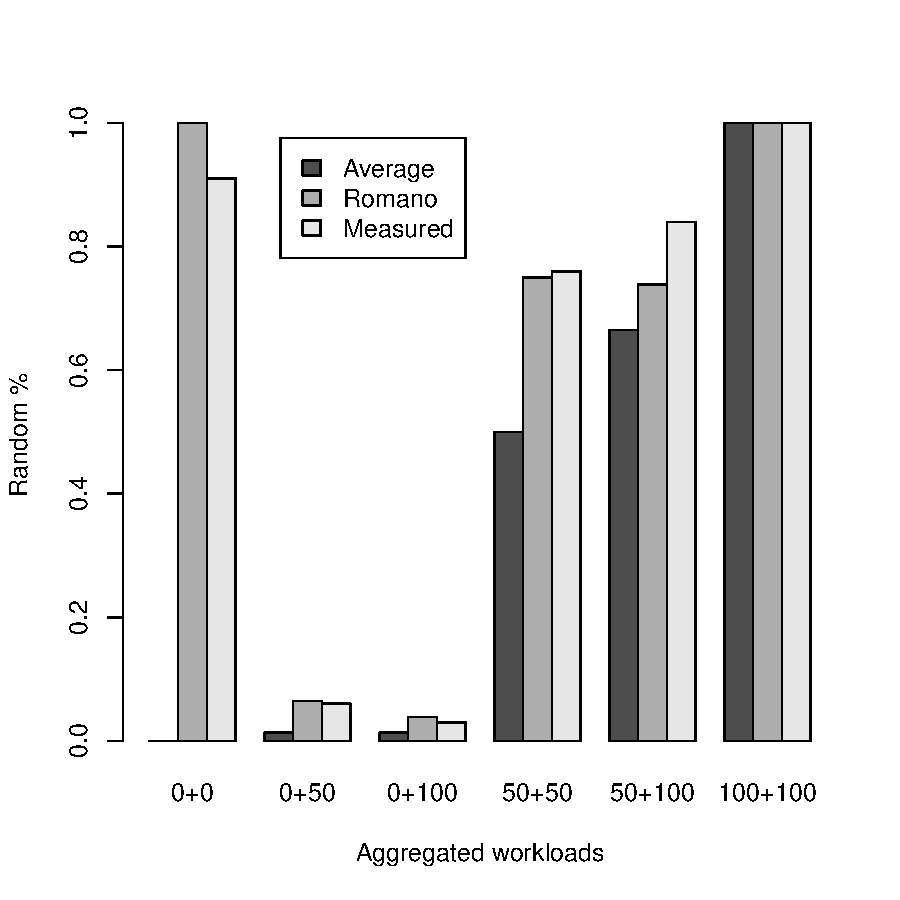
\includegraphics[width=0.8\textwidth]{figure/random_accuracy.pdf}
\captionsetup{format=myformat}
\caption{Comparison of $f_R$ and $T$ weighted average for the randomness of aggregated workloads.
Each color represents different methods.
Other characteristics are fixed at $S=4\mathit{KB}$, $\READ=100\%$ read, $\OIO=1$.
}
\label{randmix}
\end{figure}
\figurename~\ref{randmix} shows the result of $f_{\RAND}$ against simple $T$ weighted average.
The maximum and average error of doing $T$ weighted average is 100\% and 48\% respectively.
For $f_{\RAND}$ these values are 28\% and 5\% respectively.
The maximum error in both cases are when aggregating two completely sequential workloads whose resulting ${\RAND}_{\mathit{aggr}}$ has inherently high variance.

Putting it together, \emph{Romano Aggregation Model} is;
\begin{equation}\label{sumFun}
(\RAND_{\mathit{new}}, \READ_{\mathit{new}}, \SIZE_{\mathit{new}}, \OIO_{\mathit{new}}) \\
  = (f_{\RAND}({\RAND}_i, T_i), \frac{\sum_{i} {\READ}_i T_i}{\sum_{i} T_i}, \frac{\sum_{i} {\SIZE}_i T_i}{\sum_{i} T_i}, \sum_{i} {\OIO}_i)
\end{equation}
where aggregating more than 2 workloads require $f_{\RAND}$ to be recursively applied to the workloads.
In practice, this is naturally done since only a single virtual disk is migrated at a time.

\section{Romano Load Balancer}
The \emph{Romano Load Balancer} is different from traditional load balancers~\cite{gulati:2010, gulati:2011, singh:2008} in two ways.
Firstly, it optimizes the global state rather than a single storage migration.
Secondly, it is proactive.
The balancing mechanism does not wait until a overutilization is detected.
It continuously adjust the overall state whenever possible to ensure that systems are less likely to be over-utilized.
This is made possible by Romano's accurate and robust modeling techniques.

\subsection{Merit Metric}
Our load balancing goal is to minimize the overall latency while reducing the maximum latency.
To represent both aspect of our goal with a single metric, we define Romano load balancing metric of Merit~($M$) to be the form;
\begin{equation}\label{merit}
M=\left(\sum_iP_i^\alpha\right)^\frac{1}{\alpha}
\end{equation}
where $\alpha$ controls the weight on the maximum latency.
For example, if $\alpha$ is 1, $M$ is simply the sum of all latencies.
However, as $\alpha$ becomes larger, more weight is given to high latencies.
Our experiment shows that 5 is a reasonable value for $\alpha$.
However, further exploration of $\alpha$ space is left for the future work.

\subsection{Load Balancing}

\begin{algorithm}[!t]
\DontPrintSemicolon
\SetKw{updateMerit}{updateMerit}
\SetKwInOut{Input}{input}\SetKwInOut{Output}{output}
\updateMerit($W_{cand}, S_{dest}, \Phi$)
\Begin {
  $S_{src}\leftarrow getS(W_{cand}, \Phi)$\;
  $W_{src}\leftarrow getW(S_{src}, \Phi)$\;
  $W_{dest}\leftarrow getW(S_{cand}, \Phi)$\;
  $W'_{src}\leftarrow$aggregate($W_{src}-W_{cand}$)\;
  $W'_{dest}\leftarrow$aggregate($W_{dest}+W_{cand}$)\;
  $P'_{src}\leftarrow$predict($S_{src}$, $W'_{src}$)\;
  $P'_{dest}\leftarrow$predict($S_{dest}$, $W'_{dest}$)\;
  \Return{merit($P'_{all}$)}
}
\caption{Merit Update Function}\label{malgo}
\end{algorithm}

\begin{algorithm}[!t]
\DontPrintSemicolon
\SetKw{minimizeMerit}{minimizeMerit}
\SetKwInOut{Input}{input}\SetKwInOut{Output}{output}
\minimizeMerit($\Phi_i, M_i$)
\Begin{
  $\Phi\leftarrow \Phi_i$\;
  $M\leftarrow M_i$\;
  $\Phi_f\leftarrow \Phi_i$\;
  $M_f\leftarrow M_i$\;
  $K\leftarrow 0$\;
  \While{$K<K_{max}$} {
    $T\leftarrow$temperature($k/k_{max}$)\;
    $W_{cand}\leftarrow$randomChoose($W_{all}$)\;
    $S_{src}\leftarrow getS(W_{cand}, \Phi)$\;
    $S_{cand}\leftarrow$randomChoose($S_{all}-S_{src}$)\;
    $M'\leftarrow$updateMerit($W_{cand}, S_{cand}, \Phi$)\;
    \If{$G(M, M',T) >$ random()}
      {$\Phi\leftarrow$($W_{cand} \rightarrow S_{cand}$)\;
      $M\leftarrow M'$}
    \If{$M<M_f$}{
      $\Phi_f\leftarrow (W_{cand}\rightarrow S_{cand})$\;
      $M_f\leftarrow M'$\;}
    $K \leftarrow K+1$
  }
  \Return{$\Phi_f, M_f$}
}
\caption{Simulated Anealing}\label{salgo}
\end{algorithm}


\begin{algorithm}[!t]
\DontPrintSemicolon
\SetKw{loadBalance}{loadBalance}
\SetKwInOut{Input}{input}\SetKwInOut{Output}{output}
\loadBalance($\Phi_i$)
\Begin{
  $M_i \leftarrow$merit($\Phi_i$);
  $\mathit{Mlist}\leftarrow \emptyset$\;
  $(\Phi_f, M_f) \leftarrow$minimizeMerit($\Phi_i, M_i$)\;
  \ForEach{$W \in \Phi_f$}{
    \If{$getS(W, \Phi_f) \ne getS(W, \Phi_i)$}{
      $\mathit{MoveCandidate} \leftarrow W$\;
    }
  }
  \While{MoveCandidate} {
    \ForEach{$W \in$ MoveCandidate}{
      $M' \leftarrow$ updateMerit($W, getS(W, \Phi_f), \Phi_i$)\;
      append($\mathit{Mlist}, (M',W,getS(W, \Phi_f))$)\;
    }
    sortDescendingByM($\mathit{Mlist}$)\;
    $(M, W, S) \leftarrow \mathit{Mlist}[0]$\;
    Move($W$, $S$)\;
    $M_i \leftarrow $ updateMerit($W, S, \Phi_i$)\;
    $\Phi_i \leftarrow (W \rightarrow S)$\;
    $\mathit{MoveCandidate} \leftarrow \mathit{MoveCandidate}-W$\;
  }
}
\caption{Romano Load Balancing Algorithm}\label{algo}
\end{algorithm}

Romano uses \emph{simulated annealing}~\cite{kirkpatrick:1983} to optimize the overall placement and then makes moves that result in maximum reduction of $M$.
The reason for the first step is that greedy approaches used in previous works~\cite{gulati:2010, gulati:2011, singh:2008} could result in a local optimum that is far from the global optimum.
The solution cannot be greedy since any optimal sub-placement needs to be reevaluated once a new workload is added due to the aggregation function.
Adding a new data store is worse since every data store has its own performance model.
While the simulated annealing process does not necessarily result in optimal placements, it is guaranteed to be better than finding a local optimal if the algorithm can remember the best state it has seen so far~\cite{granville:1994}.

However, the resulting state may require too many workloads to be migrated.
Therefore, once the target state is defined through simulated annealing, we use a greedy method to get there.
This way, we can make moves that result in the largest reduction of $M$ while always moving towards the optimal state.
Of course, there may be a move that results in an even larger reduction but the move may prohibit the possibility of further reduction of $M$.

Algorithm \ref{algo} outlines the Romano load balancer.
In this algorithm, $\Phi$ represents the current mapping of workloads to data stores which is essentially current state of the system.
It requires two subcomponents, Alogrithm~\ref{malgo} and Algorithm\ref{salgo}. 

Algorithm \ref{malgo} simply moves a virtual disk, $W_{cand}$, to a datastore, $S_{dest}$ and recalculates the system's \emph{merit} based on the performance prediction of the source datastore, $S_{src}$, and the target datastore, $S_{dest}$.

Algorithm \ref{salgo} is the simulated annealing process where given a state and its merit, it will return a pseudo-optimal state and its merit which should be close to the global minima.
This has worked surprisingly well for this application as it will be shown in the results. 
The \emph{temperature} function and $G$ functions are taken from the earlier works on simulated annealing~\cite{kirkpatrick:1983}.
The \emph{temperature} function simply divides $k/k_{max}$ by $1.2$ every iteration.
$G$ function returns 1 if current merit is lower than previous merit so that the move is always accepted, but returns $e^{(M-M')/T}$ when current merit value is higher.
Therefore, there exists a finite chance of accepting a move even when the merit increases.
This probability decreases fast with the number of iterations and the difference between the new and old merit values.
With every iteration, the function chooses a random workload to move and a random destination data store.
New merit is calculated and the move is either rejected or accepted based on the value returned by $G$ and a random number between 0 and 1.
All our experiments required less than 200 iterations to complete.
The convergence rate of simulated annealing is difficult to predict without any structural information of the state space.
However, since we do not need the absolute minimum $M$, we can simply fix the maximum number of iterations to a reasonable number and choose the best state found.

The \emph{loadBalance} function takes the current state~($\Phi$) and calls on \emph{minimizeMerit} function to determine the pseudo-optimal mapping of $W$ on $S$.
Once the mapping is determined, it uses a greedy approach to determine which moves to execute. \emph{updateMerit} function is called on all possible moves to determine the next move.
Note that \emph{updateMerit} function executes in $O(1)$.
The process is repeated until the pseudo-optimal mapping is reached.
$getS(W, \Phi)$ represents the data store on which $W$ is mapped in current State $\Phi$ while $getW(S, \Phi)$ represents all the workloads mapped onto data store $S$ in state $\Phi$.

\emph{updateMerit} function takes the current system state~(all Workload mappings and their performance) and calculates new \emph{Merit} value.
Note that our goal is to minimize the Merit value.
The \emph{aggregate} function is \emph{Romano Aggregation Model} and \emph{predict} function is \emph{Romano Performance Model}.
Therefore, \emph{updateMerit} function is given a workload candidate to be migrated and destination data store.
New aggregated workloads are calculated and their performances are predicted.
Given the new performances of source and destination data stores, global merit is recalculated.

In practice, it is unlikely that all the moves will be carried out due to the cost involved with the migration. Furthermore, the workload themselves are going to change over time.
Therefore, Algorithm \ref{algo} will periodically rerun \emph{minimizeMerit} function and continually transition the system towards the newly found pseudo-optimal state without ever actually getting there.

\section{Results}

\subsection{Workload Aggregation}

To test the effect of workload aggregation, we need to able to generate a repeatable workload.
\begin{table}
\centering
\begin{tabularx}{0.9\textwidth}{
  X|
  >{\centering}X|
  >{\centering}X|
  >{\centering\arraybackslash}X
}
\hline
Workload      & $\mathit{IOSize}$ & $\mathit{Read\%}$ & $\mathit{Random\%}$ \\
\hline
Web File Server & 4KB             & 95\%              & 75\% \\
Web File Server & 8KB             & 95\%              & 75\% \\
Web File Server & 64KB            & 95\%              & 75\% \\
Support DB & 1MB         & 100\%             & 100\% \\
Media Streaming & 64KB            & 98\%              & 0\% \\
SQL Server Log  & 64KB            & 0\%               & 0\% \\
Web Server Log  & 8KB             & 0\%               & 100\% \\
OLTP DB         & 8KB             & 70\%              & 100\% \\
Exchange Server & 4KB             & 67\%              & 100\% \\
Workstation     & 8KB             & 80\%              & 80\% \\
VOD             & 512KB           & 100\%             & 100\% \\
\hline
\end{tabularx}
\captionsetup{format=myformat}
\caption{Workload characteristics suggested by Wang~\cite{wang:2009}.
These workloads are used to ensure repeatable experiments.
}
\label{test_wl}
\end{table}
We use the workload settings shown in \tablename~\ref{test_wl} to simulate the real workloads.
Previous works have shown that synthetic workloads do a good job of representing real workload's performance characteristics when the parameters are extracted from the real workloads~\cite{tarasov:2012, park:2011}.

All possible combinations of two workloads were chosen from the 11 workloads shown in \tablename~\ref{test_wl} resulting in 55 combinations.
In Romano workload characteristics space, aggregating 2 workloads and 3 workloads are the same since the aggregation process is commutative and associative.
$\OIO$ was randomly assigned from 1 to 3. The test was repeated on two data stores for which the Romano model performed worst (see \figurename~\ref{rdRomano}).

The workload aggregation method used in Pesto~\cite{gulati:2011} is to average their workload metric $\omega$ weighted by $OIO$.
To isolate the effect of workload aggregation, we average individual workload characteristics weighted by $\OIO$ and use \emph{Romano Performance Model} to predict the latency.
\begin{figure}[!t]
\centering
\subfloat[Sample of latency prediction]{\label{aggrPred}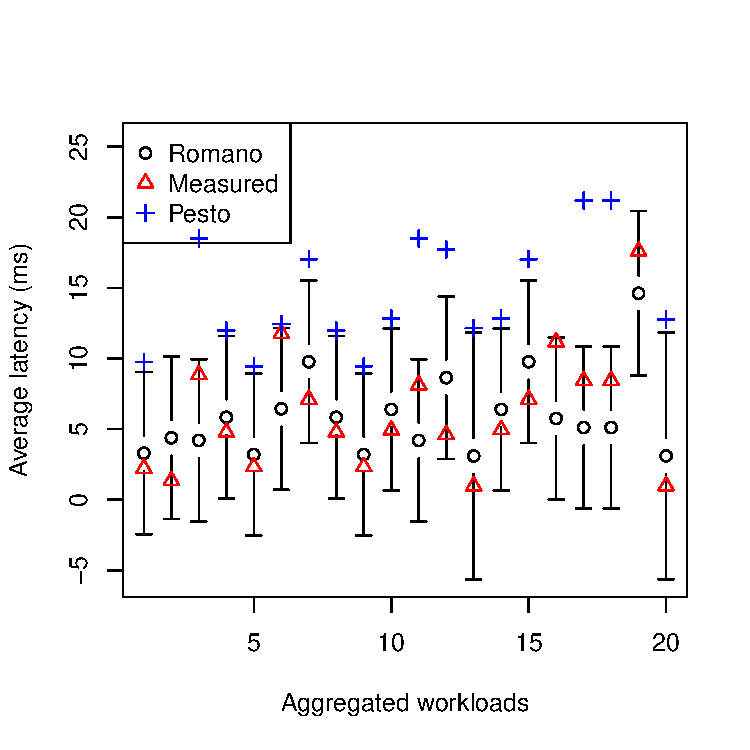
\includegraphics[width=0.625\textwidth]{figure/aggr_result.pdf}}
\subfloat[Residuals box plot]{\label{aggrRes}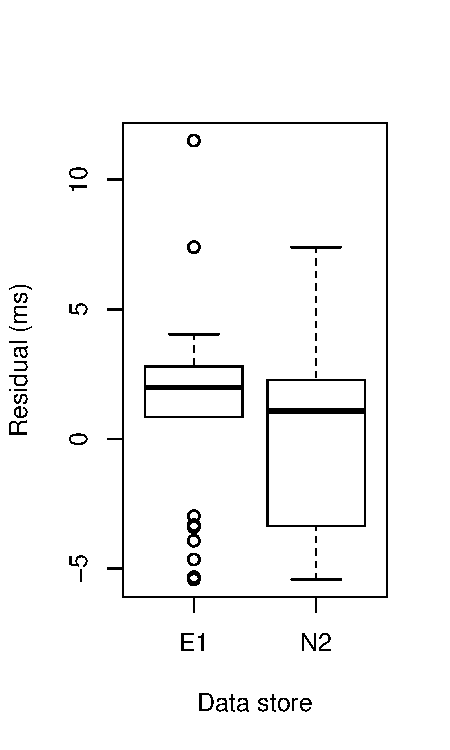
\includegraphics[width=0.375\textwidth]{figure/aggr_error.pdf}}
\captionsetup{format=myformat}
\caption{Result of workload aggregation.
Two Workloads from \tablename~\ref{test_wl} were placed randomly across two data stores, E1 and N2.
\figurename~\ref{aggrPred} shows 20 randomly sampled results from 110 placements on both data stores (55 each).
\figurename~\ref{aggrRes} shows the residual of all 55 placements on E1 and N2.
}
\label{aggr}
\end{figure}

The result is shown in \figurename~\ref{aggr}.
\figurename~\ref{aggrPred} shows the latency from 20 randomly selected experiments as well as the prediction interval of Romano.
Only in 1 case, Romano failed to capture the latency within its prediction interval.
In fact, only 3 out of 110 cases (2.7\%) showed Romano failing to capture the measure latency.
This is better performance than specified 5\% confidence level.
We believe that this is due to the unbiased nature of Romano residual shown in \figurename~\ref{rdRomano}.
As the workloads are aggregated, the residuals ($\epsilon$) of \emph{LQ-slope} prediction, used for workload aggregation, are more likely to cancel each other out.

The accuracy of Pesto's approach of $\OIO$ weighted average does not seem too bad at first but there are some cases where the prediction won't even register on the \figurename~\ref{aggrPred} (workload 2 and 16).
This is especially true if the workloads running together are highly skewed such that one workload has much higher throughput than the other.
This verifies our assumption that the workload should be aggregated based on its throughput rather than $\OIO$.
his is especially true if the workloads running together are highly skewed such that one workload has much higher throughput than the other.
This verifies our assumption that the workload should be aggregated based on its throughput rather than $\OIO$.
\figurename~\ref{aggrPred} also shows that while Pesto consistently overpredicts the aggregated latency, Romano residuals are more unbiased shown in \figurename~\ref{aggrRes}.

Another interesting result was that all 3 cases where Romano failed were observed on E1 data store.
This is as expected from the amount of outliers shown in \figurename~\ref{aggrRes}.
We believe that amount of uncertainty introduced by workload aggregation is different on each data store.
We leave the further investigation to future work.

\subsection{Load Balancing Using Romano}

\begin{figure}[!t]
\centering
\subfloat[Initial data stores latencies.]{\label{lb_init}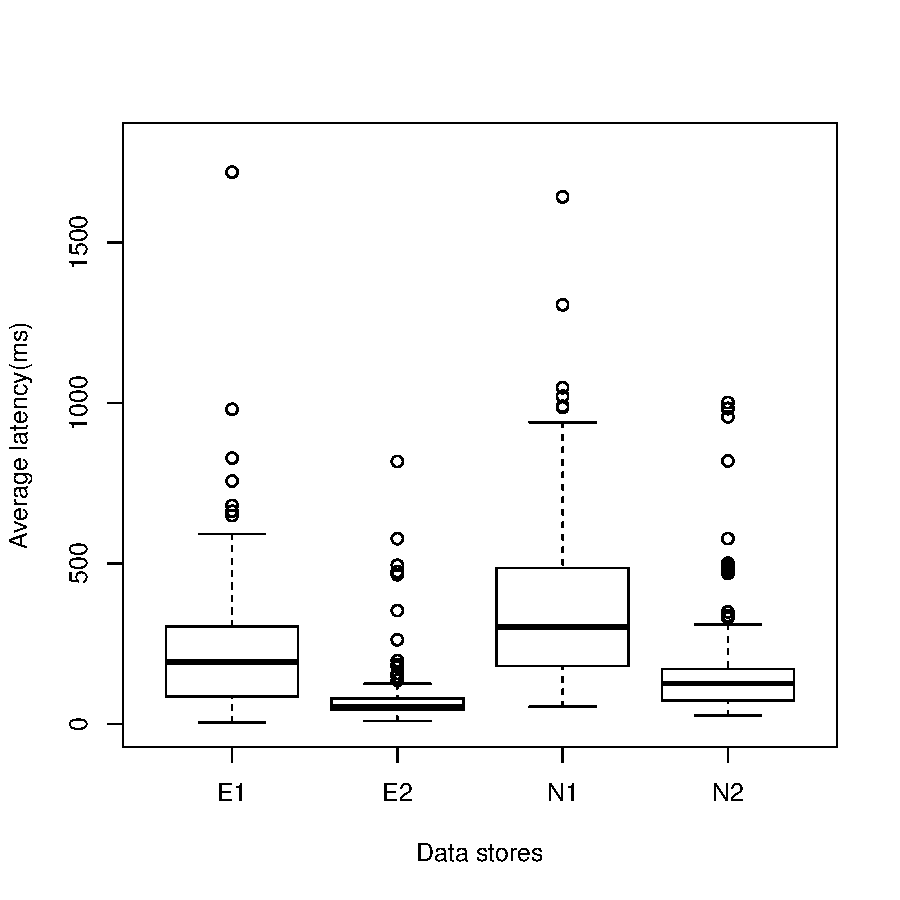
\includegraphics[width=0.7\textwidth, clip, trim=0 0.2in 0in 0.5in]{figure/initial_datastore_latency.pdf}}\\
\subfloat[Result of Basil load balancing]{\label{lb_basil}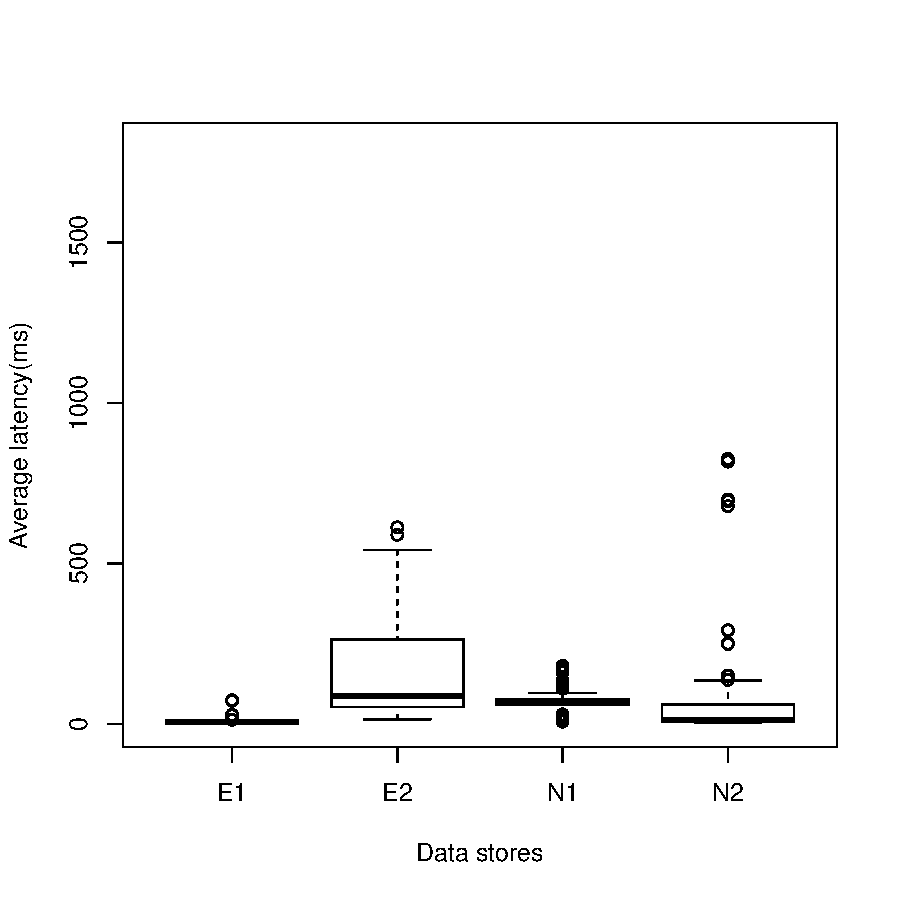
\includegraphics[width=0.7\textwidth, clip, trim=0 0.2in 0in 0.5in]{figure/basil_datastore_latency.pdf}}\\
\end{figure}

\begin{figure}[!t]
\ContinuedFloat
\centering
\subfloat[Result of Romano load balancing.]{\label{lb_after}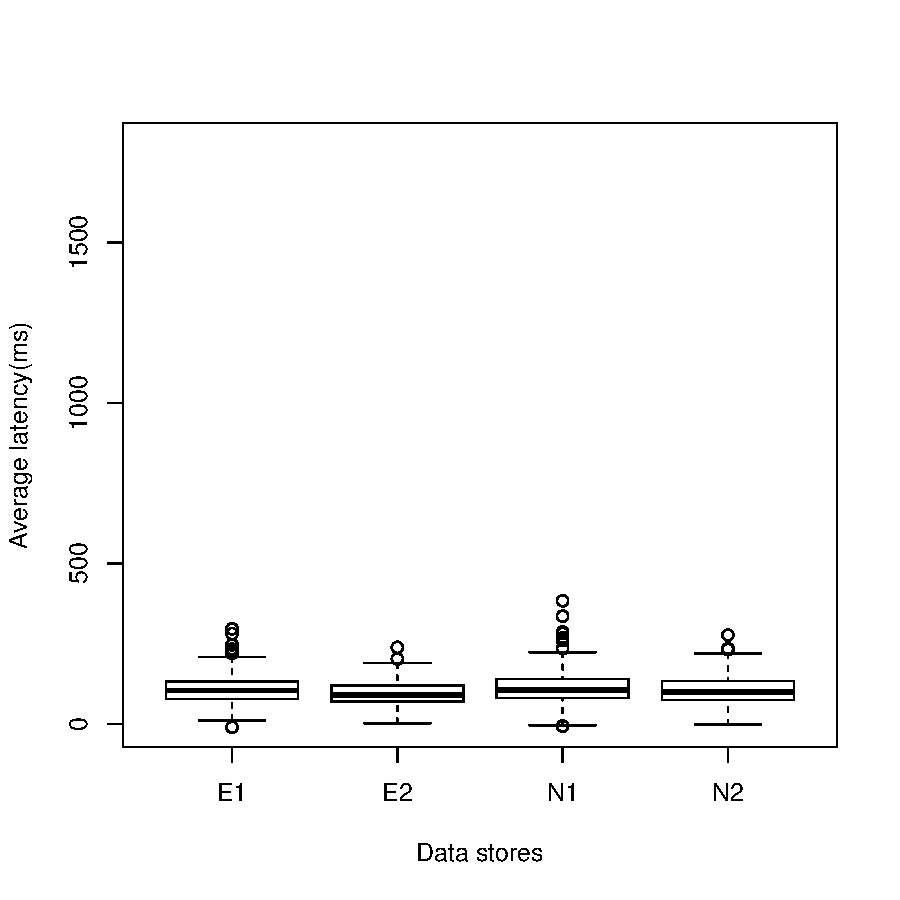
\includegraphics[width=.7\textwidth, clip, trim=0 0.2in 0in 0.5in]{figure/romano_datastore_latency.pdf}}
\captionsetup{format=myformat}
\caption{Boxplot of average data store latencies on 50 different test cases.
Each test randomly placed 8-14 workloads from \tablename~\ref{test_wl} (allowing repetition) on 4 data stores.
Basil's greedy approach is compared with Romano's random optimization technique.
}
\label{load_bal}
\end{figure}

In this section we randomly placed 8-14 workloads from \tablename~\ref{test_wl} allowing repetition on 4 data stores.
Romano load balancing algorithm from Algorithm 1 was ran to optimize the data placement by moving a single virtual disk at a time.
The experiment was repeated 50 times.

\figurename~\ref{load_bal} shows the aggregated result of load balancing using Basil and Romano.
It should be noted that the load balancing algorithm deployed by Basil and Pesto are the same.
Both Basil and Romano does a good job of reducing the average latency by 47\% and 52\% respectively.
However, the variance is reduced by 82\% by Romano while Pesto reduces it by 37\%.
Most importantly, the maximum latency observed was reduced by 78\% with Romano while only 21\% by Pesto.

There are two factors which result in improved performance by Romano.
The first is the more accurate modeling.
Both Pesto and Basil assume that there exists only a constant performance difference between different data stores for any given workload.
Therefore, it has tendency to move virtual disks to a data store that is more powerful regardless of the workload.
Furthermore, their aggregation model is based on the outstanding IOs only.
This allows workload that do not performance well together to be placed on a single data store.
The result of these inaccuracies in the model forces the load balancing algorithm to place more workloads on the powerful data stores.
In fact 51\% of all the moves by Pesto were made to E2 data store compared to 28\% for Romano.
\figurename~\ref{lb_basil} shows that resulting E1 and N1 latencies are smaller than that of Romano while E2 and N2 exhibit large latencies that we would like to avoid.
In fact, Basil does not place any workload on E1 90\% of the time even though E1 actually has lower latency for most workloads than N1 as shown in \figurename~\ref{slm}.

The second factor is the load balancing algorithm itself.
Basil and Pesto uses a greedy approach~\cite{gulati:2010} which terminates the algorithm once no beneficial moves are found.
Romano uses simulated annealing to find the pseudo optimal placement first and than uses greedy approach to get to the optimal placement.
This allows Romano to avoid moves that may result in maximum benefit but prohibits any further moves that may provide additional benefits.

\begin{figure}[!t]
\centering
\subfloat[Basil]{\label{basil_mv}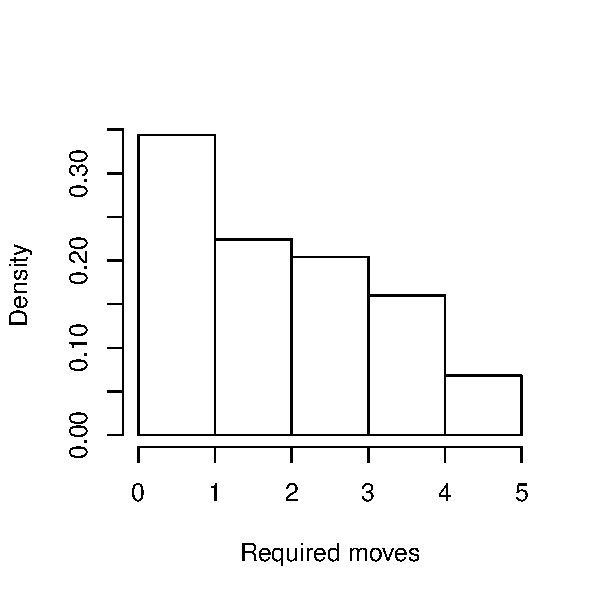
\includegraphics[width=0.5\textwidth]{figure/basil_required_moves.pdf}}
\subfloat[Romano]{\label{romano_mv}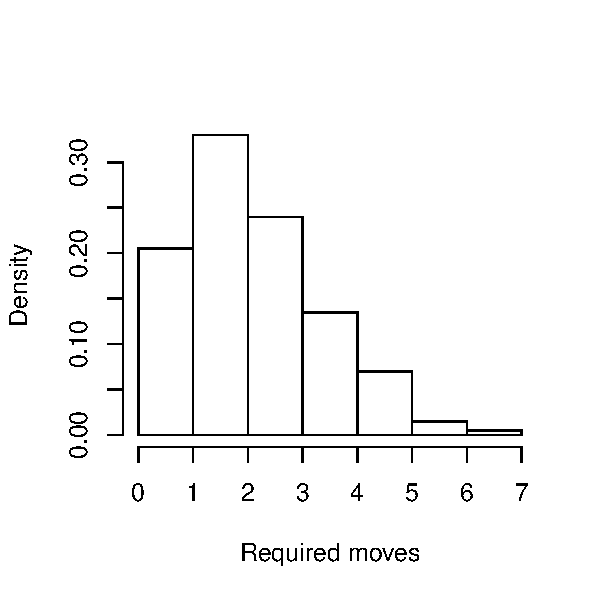
\includegraphics[width=0.5\textwidth]{figure/romano_required_moves.pdf}}
\captionsetup{format=myformat}
\caption{
The distribution of number of moves resulting from Basil and Romano.
}
\label{moves}
\end{figure}

\begin{figure}[!t]
\centering
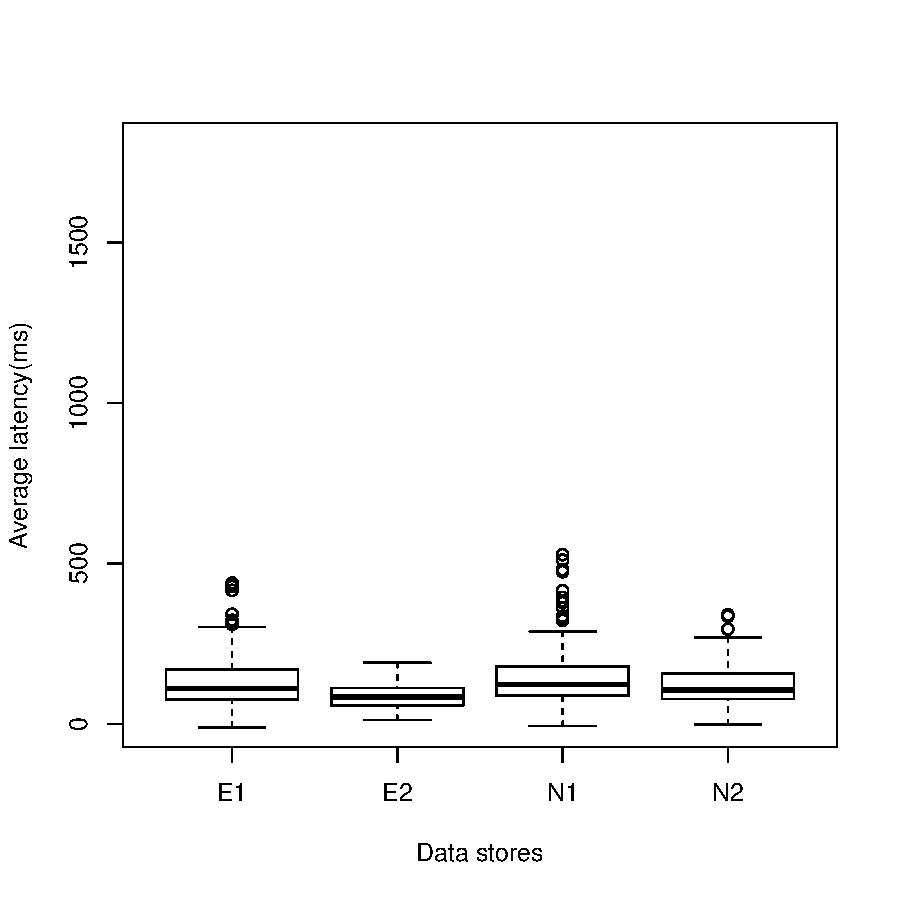
\includegraphics[width=0.8\textwidth]{figure/romano_latency_2moves.pdf}
\captionsetup{format=myformat}
\caption{Data store latencies after maximum of 2 moves with Romano.}
\label{two}
\end{figure}

One limitation of this approach is that it does require more moves to be made.
\figurename~\ref{moves} shows the number of moves required for Basil and Romano.
On average Basil requires $2.2$ moves where as Romano required $2.6$.
Storage migration is expensive and should avoided if possible.
However, we show that even if we limit the maximum number of moves to 2, Romano still out performs Basil as shown in \figurename~\ref{two}.
This is due to the greedy approach in which Romano chooses moves once the pseudo-optimal placement is identified.

\begin{figure}[!t]
\centering
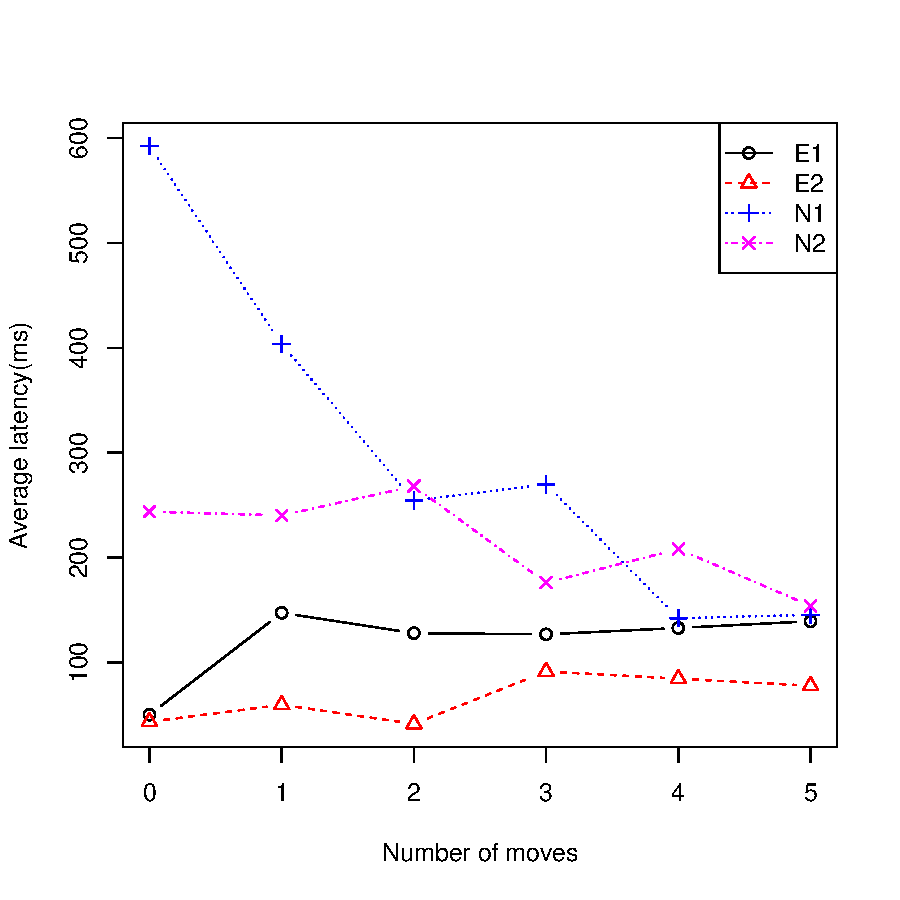
\includegraphics[width=0.8\textwidth]{figure/23latency_reduction.pdf}
\captionsetup{format=myformat}
\caption{Typical Romano load balancing process with large number of moves.}
\label{proc}
\end{figure}

\figurename~\ref{proc} shows an example of latency changes for a single test case.
It is shown that most critical balancing is done within the first couple of moves.
%\nohhyun{5.4  About the pseudocode, why is D removed from the list when a virtual disk is assigned to it?  Can’t a data store handle more than one virtual disk depending on its performance characteristics?}
~
\section{Conclusion}\label{CONCL}
We have presented Romano, a load balancing framework for virtual disks
on heterogeneous storage systems. The kernel of Romano is a performance
predictor given a set of parameters that characterize the workloads and
the storage devices. We have shown that Romano can outperform
previous systems with same goals by up to 80\% in prediction
accuracy. This increased accuracy results in 78\% reduction in maximum
latency observed and 82\% reduction in variance while load balancing.

At a deeper level, Romano contributes a recognition that there is
inherent noise in storage system performance that is not easily dealt
with. Romano is capable of capturing this noise within the prediction
interval. As more data is gathered there is higher confidence that the
prediction interval will contain the measured latency.

Another key contribution of Romano is quantification of effect of
various workload characteristics and their interaction on heterogeneous
storage devices.
We have shown that the performance differences between data stores cannot be described with a single number. More specifically, we have shown that the storage performance must be described in terms of the workload.

The last contribution follows the second contribution. Since the performance of storage systems effectively change with the workload, the load balancing problem is no longer a bin-packing problem as previously believed.
Therefore we present a probabilistic approach to finding a pseudo-optimal mapping of workloads to the data stores.
It is important to mention that probabilistic approach is only used to find the final state of the system and the moves are actually made greedily to speed up the convergence and minimize the number of moves that has to be made.

We believe that Romano not only provides means for more efficient load
balancing but also in many other areas such as QoS management, power management and performance tunning in tiered storage.

Whereas Romano raises the bar on the accuracy of practical modeling
techniques, there remain ample opportunities for improvements in
future work. Better interference modeling between workloads when they
are placed on same data store is one such area where we are making
good progress. Another work in progress is to come up with a better
set of workload characteristics such that the workload description can
be more complete.
~
